
\chapter{Reference Model Construction}
%%%%%%%%%%

This chapter conceptions the process reference model and is central part of this thesis. In order to discuss particular processes, the framework itself needs to be discussed. What follows is the discussion of processes, which puts special emphasis on design decisions, \viz \textit{how} to model certain aspects with constructs of the language icebricks. 

\begin{itemize}
	\item Approach from Case advanced to the model itself
	\item ECIS model schemata
	\item type / instance : hybride leistungsbündel
\end{itemize}

	%%%%%%%%%%
	deloitte W14: managing change dispute:::: innovation und so... wichtig für begründung des frameworks
	\section{Process Framework}
	
	\citeauthor{Meise2001} defines a framework as \enquote{an ordering relevant elements and relationships on a high level of abstraction. [...] Purpose is to give an overview about an original and to support structuring of elements and relationships on lower detail levels} \citep[62]{Meise2001}. Drawing further on his work, which especially targets framework design in process-oriented organizations, the proposed procedure for construction is adopted (\Fig \ref{fig:meise}). Differences to his approach arise, as the reference model should display as as-is state of the domain and does not follow goals of reorganization set by a specific company. Therefore, the \textit{organization} represents a fictive BPO provider in CRM in the following, which captures generic aspects of the domain. The construction is split into two components. The structural part first encompasses strategic and fundamental reflections, while the graphical component transfers these into a visual form that supports communication.

	\begin{figure}[caption={procedure for framework construction}, label={fig:meise}]
		{	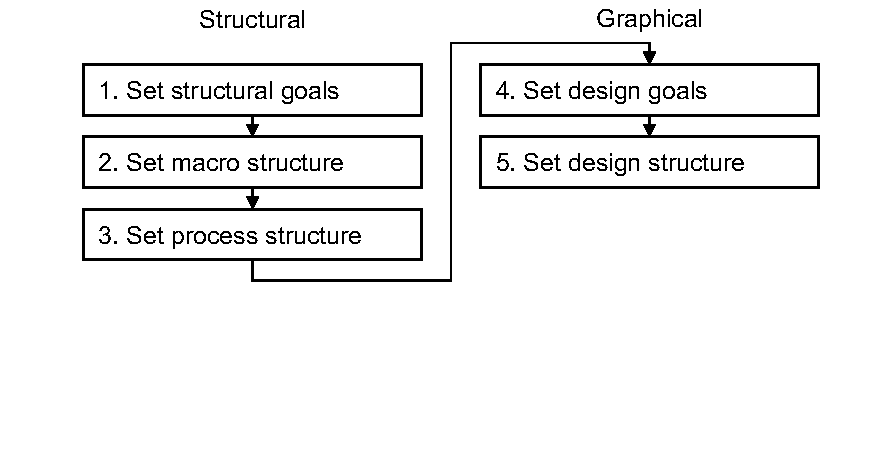
\includegraphics[width=.8\textwidth]{figures/framework-meise.pdf}}
		\hspace{6.2cm}	SOURCE:  adapted from \citep[\p{122}]{Meise2001}
	\end{figure} 
	
	\textit{Ad 1. Set structural goals}
	
	Modeling is no end in itself and different purposes require different models. Theoretically speaking, purpose of this research is to create an artifact that generates utility and tackles a problem in the real-world.  Previously identified problems (\ref{sec:proide}) lead to objectives (\ref{sec:solobj}) which are to be faced with the process reference model in general and its framework in particular. The existence of general (organizational) and stakeholder-related objectives requires the framework to bring together both ends, as it is the basis of the model. 
	
	
	\textit{Ad 2. Set macro structure}
	
	A framework, as a strategic tool, incorporates concepts of strategy. One can name two perspectives, namely a market- or resource-based view of strategy, which are directed externally or internally, respectively. They are not independently of each other, but their interplay is seen as an important factor in strategic decision making. \cite{becker2004handelsinformationssysteme} note, that standardization in keeping with reference model application has contra-productive effects on strategic competitive advantages. This argument is true, when the reference model is used as a application model. The application of the reference should incorporate strategic characteristics of the company, which implies that this reference model framework can only capture a strategic orientation as perceived useful by the author. 
	
	The market-based view follow the structure-conduct-performance paradigm, that explains success of a company through external factors in the industry. \cite{porter1980} formulated the so called five-forces model, which describes bargaining power of suppliers (1), threat of substitutes (2), bargaining power of buyers (3), threats of new entrants (4) and industry rivalry (5) as determinants of competition. Applying these two the BPO domain, a trivial substitute for outsourced services is the return of services inside the parent organization. Further, the substitution of customer services through automation may render outsourcing obsolete. The bargaining power of suppliers and buyers can be loosely mapped to clients and customers. While clients as suppliers clearly influence the provider directly, customers show less of this influence on the outsourcing provider. As the provider takes an intermediate position between client and customer (\cf \Fig \ref{fig:bpochain}), their acting is always in connection with the client. However, an assessment of outsourced service quality puts pressure originating from the customer on the provider, which in turn will also be judged by the client. The entry of new players on the market (4) can be tackled by barriers, that go back to competitive advantages of differentiation or cost-leadership. While the latter is especially causing fierce competition in low-wage regions that realize offshore-outsourcing, outsourcing players in CRM that feature more profound services, lean towards a differentiation strategy. This can also be stated for Arvato. Lastly, industry rivalry among players in the BPO CRM market is also influenced by the aforementioned generic strategies, to position established companies. A framework adopts market-based aspects through accounting for markets or segments therein. These are accompanied by business units or processes that relate to this external environment. 
	
	The resource-based view of strategy analyzes internal strengths and weaknesses. Resources are bundled to form capabilities and should be rare, inimitable, create value and be non-substitutable. Due to asymmetries of resources, competitive advantages are enabled. The identification of capabilities of CRM BPO providers (\cf \ref{sec:bpocrmis}: operational and business development capabilities) can only be done on a generic level for the reference model. Application necessitates specifying the framework to conform to company-specific capabilities.  The operational capability should reflect the operational process component in CRM (\cf \ref{crmprocessfr}), and service delivery from the outsourcing side (\cf \ref{app:provproc}). Business development, \ie understanding and addressing client needs, misses a pendant in an isolated CRM view, but can be put in relation to delivery management in the outsourcing model. 
	
	Putting both views together emphasizes the client and customer market environment and two capabilities, that relate to these markets. Towards the client side, providers are criticized by clients for being too reactive instead of proactive (49\%), delivering poor service quality (48\%) and lack of innovation (37\%) \citep{deloitte2014outsourcing}. While the first point of criticism addresses the client relationship, the other two are directed towards the service itself. Looking at the constituents of \acrshort{CRM}, the people, process, technology split draws a line to the resource-based view, as these three resources need to be developed and captured to enable superior service provision for clients. Apart from the  \acrshort{CRM} view, these three also have their own meaning in \acrshort{BPO}. The importance of processes in  \acrshort{BPO} is obvious. The people component can be interpreted here as the provision of manpower and their training for services; (information) technology as an enabler of outsourcing (\cf \ref{sec:bpo}) . 
	
		
	\textit{Ad 3. Set process structure}
	
	Given that the process shows processes, the structural split of people, processes and technology is hardly meaningful, as two aspects of  \acrshort{CRM} or \acrshort{BPO} would be left out. Drawing from the BPO chain and the identified stakeholders enables another categorization that leaves room for design choices, while capturing generic aspects of  \acrshort{BPO}. As \acrshort{BPO} is the framing construct and  \acrshort{CRM} one use of it, this order is to be prioritized.  
	
	\textit{Ad 4. Set design goals}
	
	\textit{Ad 5. Set design structure}
		
	%%%%%%%%%%
	\begin{itemize}
		\item meise 2001
	\end{itemize}
	%%%%%%%%%%
	\section{Internal Services}
	%%%%%%%%%%
	%%%%%%%%%%
	\subsection{...}
	%%%%%%%%%%
	%%%%%%%%%%
	\section{Client Services}
	%%%%%%%%%%
	%%%%%%%%%%
	\subsection{...}
	%%%%%%%%%%
	%%%%%%%%%%
	\section{Customer Services}
	This analysis is necessary due to the complex and highly variable processes in Customer Service. Process Identification for Customer Service in the field of the After Sales Service as a Basis for “Lean After Sales Service”
	
	im hippner buch it automation chapter für self service!
	%%%%%%%%%%
	Self Service: Servitization paper 1988!
	%%%%%%%%%%
	\subsection{...}
	%%%%%%%%%%
	%%%%%%%%%%
